\documentclass[10pt,aspectratio=169]{beamer}
\usetheme{Execushares}

\usepackage[algoruled]{algorithm2e}

\renewcommand{\raggedright}{\leftskip=2pt \rightskip=2pt plus 0cm} 


%\usepackage[maxcitenames=2,backend=biber,sorting=ynt]{biblatex}
%\addbibresource{lubric2013.bib}

\newcommand{\citex}[1]{\citeauthor{#1}, \citeyear{#1}}

\usepackage{multirow} %multifilas

\usepackage{booktabs}

\usepackage{multimedia}

\usepackage{bm}

\graphicspath{{figs/}}

\usepackage{color}
\usepackage{amsmath,amsthm,amsfonts}

\newcommand{\hzerooneOm}{{H_0^1(\Omega)}}
\newcommand{\hzerooneom}{{H_0^1(\omega)}}
\newcommand{\honeOm}{{H^1(\Omega)}}
\newcommand{\honeom}{{H^1(\omega)}}
\newcommand{\lpOm}[1]{{L^{#1}(\Omega)}}
\newcommand{\lpom}[1]{{L^{#1}(\omega)}}
\newcommand{\parder}[2]{\frac{\partial #1}{\partial #2}}
\newcommand{\pardertwo}[2]{\frac{\partial^2 #1}{\partial #2^2}}
\newcommand{\parderD}[2]{\frac{\mbox{D} #1}{\mbox{D} #2}}
\newcommand{\parderDtwo}[2]{\frac{\mbox{D}^2 #1}{\mbox{D} {#2}^2}}

\newcommand{\tm}[1]{\textnormal{\scriptsize{#1}}}
\newcommand{\pcc}{p_{\textnormal{\scriptsize{cc}}}}
\newcommand{\pcav}{p_{\textnormal{\scriptsize{cav}}}}
\newcommand{\peq}{p_{\textnormal{{eq}}}}
\newcommand{\Req}{R_{\textnormal{{eq}}}}

\newcommand{\hzero}{H^1_0\left(\Omega\right)}
\newcommand{\hone}{H^1\left(\Omega\right)}
\newcommand{\honedual}{H^{-1}\left(\Omega\right)}
\newcommand{\sobz}[2]{W_0^{#1,#2}\left(\Omega\right)}
\newcommand{\sob}[2]{W^{#1,#2}\left(\Omega\right)}
\newcommand{\cont}{C\left(\bar{\Omega}\right)}
\newcommand{\norm}[2]{\left\lVert#1\right\rVert_{#2}}
\newcommand{\Sp}[1]{\textnormal{Sp}\left(#1\right)}
\newcommand{\Vp}[1]{\textnormal{Vp}\left(#1\right)}

\DeclareMathOperator*{\essinf}{ess\,inf}

\setbeamertemplate{theorems}[numbered]
\title{New models and Numerical Methods in Hydrodynamic Lubrication}
\author{Alfredo Jaramillo}
\date{February 7, 2019}

\newenvironment{nalign}{
	\begin{equation}
	\begin{aligned}
}{
	\end{aligned}
	\end{equation}
	\ignorespacesafterend
}

\newenvironment{nalign*}{
	\begin{equation*}
	\begin{aligned}
}{
	\end{aligned}
	\end{equation*}
	\ignorespacesafterend
}
\usepackage{color}

\newcommand{\hzero}{H^1_0\left(\Omega\right)}
\newcommand{\hone}{H^1\left(\Omega\right)}
\newcommand{\honedual}{H^{-1}\left(\Omega\right)}
\newcommand{\sobz}[2]{W_0^{#1,#2}\left(\Omega\right)}
\newcommand{\sob}[2]{W^{#1,#2}\left(\Omega\right)}
\newcommand{\cont}{C\left(\bar{\Omega}\right)}
\newcommand{\norm}[2]{\left\lVert#1\right\rVert_{#2}}
\newcommand{\Sp}[1]{\textnormal{Sp}\left(#1\right)}
\newcommand{\Vp}[1]{\textnormal{Vp}\left(#1\right)}

\DeclareMathOperator*{\essinf}{ess\,inf}

\setbeamertemplate{theorems}[numbered]

\setcounter{showSlideNumbers}{1}

\begin{document}
\setcounter{showProgressBar}{0}
\setcounter{showSlideNumbers}{1}

\frame{\titlepage}

%==============================================================


\begin{frame}
\frametitle{Layout}
\tableofcontents[hideallsubsections]
\end{frame}

\section{Introduction}
\subsection{Motivation}

%==============================================================

\begin{frame}
\frametitle{The Piston-Ring-Cylinder device}
\vspace*{0.5cm}
\begin{figure}\hspace*{-0.3cm}
	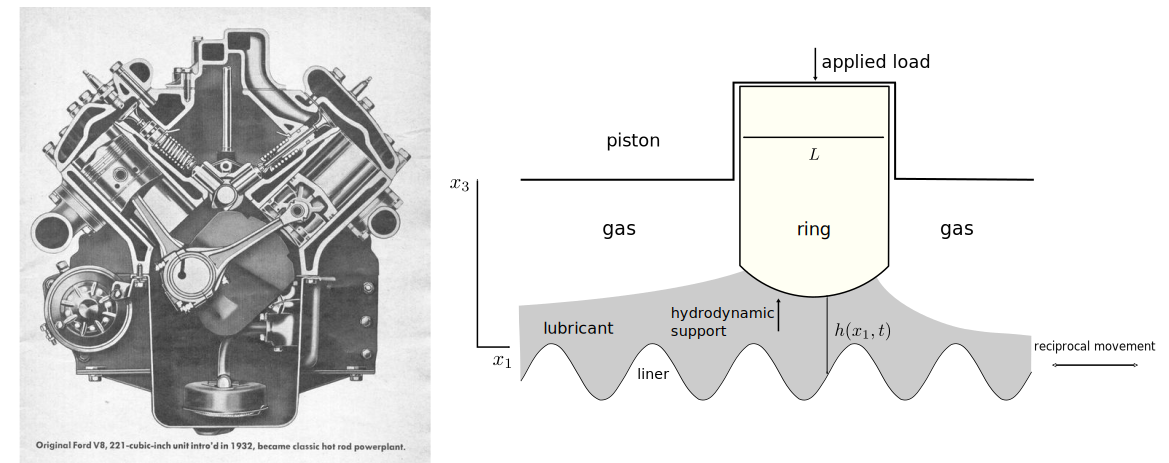
\includegraphics[scale=0.49]{esquema_experimentoF.pdf}
\end{figure}
\end{frame}

%==============================================================
\begin{frame}
\frametitle{The Journal Bearing}
\vspace*{0.7cm}
\begin{figure}
	\centering
	\includegraphics[scale=0.55]{journal_bearing.pdf}
\end{figure}

\end{frame}

%==============================================================
\begin{frame}
\frametitle{Cavitation and water treatment}
\vspace*{0.5cm}
\begin{minipage}{\linewidth}
\begin{figure}
	\includegraphics[scale=0.6]{water_treatment.pdf}
\end{figure}
\end{minipage}
\end{frame}


%==============================================================

\subsection{Reynolds Equation and cavitation modeling}

%==============================================================

\begin{frame}
\frametitle{The Reynolds Equation}\bigskip
To look for the hydrodynamical pressure $p$ such that
\begin{align*}
\nabla \cdot \left( \frac{\rho h^3}{12\,\mu} \nabla p \right)- \frac{U}{2}\parder{\rho h }{x_1} &=\parder{\rho h }{t}, &&\text{in } \Omega\subset \mathbb{R}^2,\\
p&=p_\partial,&&\text{on } \partial \Omega.
\end{align*} 
\begin{itemize}
	\item $h$: gap between the surfaces;
	\item $U$: surfaces' relative velocity;
	\item $\rho$, $\mu$: fluid density and viscosity resp.;
	\item $p_\partial\in \mathbb{R}$.
\end{itemize}

\begin{center}
	but cavitation must be considered: $\rho=\rho(p)$
\end{center}
\end{frame}

%==============================================================

\begin{frame}
\frametitle{Observation of cavitation in a Journal Bearing}
\vspace*{1.0cm}
\begin{figure}
	\centering
	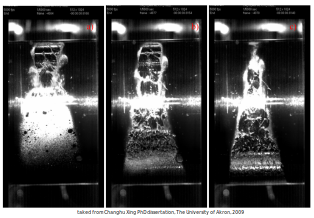
\includegraphics[scale=0.3]{cavitation_journal_bearing0.pdf}
\end{figure}
\end{frame}

%==============================================================

\begin{frame}[noframenumbering]
\frametitle{Observation of cavitation in a Journal Bearing}
\vspace*{1.0cm}
\begin{figure}
	\centering
	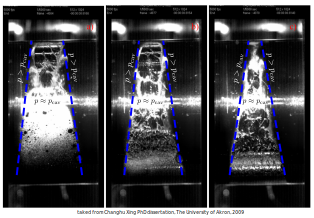
\includegraphics[scale=0.3]{cavitation_journal_bearing.pdf}
\end{figure}
\end{frame}

%==============================================================

\begin{frame}
\frametitle{The Elrod-Adams cavitation model}
\vspace*{1.0cm}
To look for the fields $p\geq p_{\text{cav}}$ and $0\leq \theta \leq 1$ such that: $$Q=\frac{h^3}{12\,\mu} \nabla p - \frac{U}{2}h\theta \, \hat{e}_1,$$ accomplishes (+ b.c.): $$\text{div} \left( Q \right) =\parder{h\theta }{t}\qquad \mbox{and}\qquad p(1-\theta)=0 \qquad \mbox{in }  \Omega.$$

\begin{figure}
	\centering
	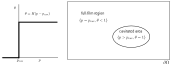
\includegraphics[scale=0.6]{cavitation_omega.pdf}
\end{figure}
\end{frame}

%=============================================================

\section{Non-Homogeneous boundary conditions for pressure}
\subsection{The separation boundary}
\begin{frame}
\tableofcontents[
currentsection,
currentsubsection,
subsectionstyle=show/shaded/hide
]
\end{frame}

%=============================================================
\begin{frame}
\frametitle{Separation boundary in a Piston-Ring}
\vspace*{1.0cm}
\begin{figure}
	\centering
	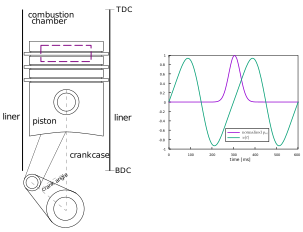
\includegraphics[scale=1.2]{piston-ring-liner.pdf}
\end{figure}
\end{frame}


%=============================================================
\begin{frame}
\frametitle{Separation boundary in a Piston-Ring}
\vspace*{1.0cm}
\begin{figure}
	\centering
	\includegraphics[scale=0.8]{cav_ring1.pdf}
	\caption{\color{ExecusharesGrey}\tiny Author: Dellis, P. 10th International Symposium on Cavitation - CAV2018}
\end{figure}
\end{frame}

%=============================================================
\begin{frame}[noframenumbering]
\frametitle{Separation boundary in a Piston-Ring}
\vspace*{1.0cm}
\begin{figure}
	\centering
	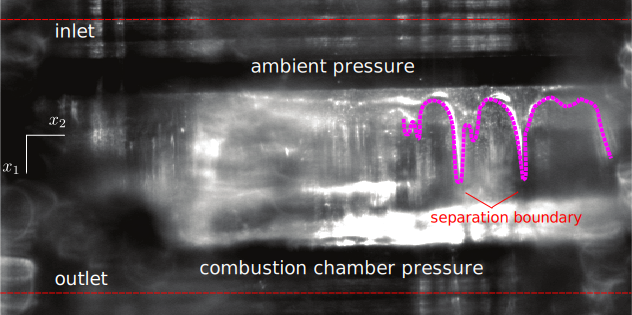
\includegraphics[scale=0.8]{cav_ring2.pdf}
		\caption{\color{ExecusharesGrey}\tiny Adapted from the work of Dellis, P.}
\end{figure}
\end{frame}

%=============================================================
\begin{frame}
\frametitle{Separation boundary in a Piston-Ring}
\vspace*{1.0cm}
\begin{figure}
	\centering
	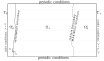
\includegraphics[scale=1.0]{omega_piston_extension_elrod.pdf}
\end{figure}
\end{frame}

\subsection{Extension of the Elrod-Adams model}
\begin{frame}
\tableofcontents[
currentsection,
currentsubsection,
subsectionstyle=show/shaded/hide
]
\end{frame}
%=============================================================
\begin{frame}
\frametitle{Extending the Elrod-Adams model}
\vspace*{1.0cm}
To look for the fields $p(\textbf{x},t)$ and $\theta(\textbf{x},t)$, $\textbf{x}\in\Omega$ and $t\in[0,t_\textnormal{f}>0]$, such that
\begin{align*}
\nabla\cdot \left( \frac{h^3}{12\,\mu} \nabla p \right)-\frac{\bar{U}}{2}\parder{}{x_1}\left(h\theta\right) &=\parder{h\theta }{t} &&\text{in } \Omega\\
p&\geq T(\theta)&&\text{in } \Omega\\
0\leq \theta &\leq 1&&\text{in } \Omega\\
(p-T(\theta))(1-\theta)&=0 && \text{in } \Omega\\
p &= 0 && \text{on } \Gamma_0\\
p &= \pcc && \text{on } \Gamma_+\\
\theta &= \theta_{\textnormal{in}} && \text{on } \partial\Omega
\end{align*} 
This corresponds to the classical Elrod-Adams model for $T\equiv 0$ and $\pcc=0$.
\begin{equation*}
(T\theta)(\mathbf{x})=
\begin{cases}
\pcc(t)  & \text{ if } \mathbf{x}\in \Omega_0^\textnormal{r}\\
0 				& \text{ if } \mathbf{x} \in \Omega_0'\cup \Omega_+
\end{cases}
\end{equation*}
\end{frame}

\subsection{Numerical scheme}
\begin{frame}
\tableofcontents[
currentsection,
currentsubsection,
subsectionstyle=show/shaded/hide
]
\end{frame}
%=============================================================
\begin{frame}
\frametitle{Discretization}
By means of Finite Volumes one gets the system
\begin{align*}
a^{00}_{i,j}\,p^n_{i,j}+e^{00}_{i,j}\,\theta^n_{i,j} &= C_{i,j}(\bm{p}^n,\bm{\theta}^n)\\
p_{i,j}^n&\geq T\left(\bm{\theta}^n\right)_{i,j}\\
0\leq \theta_{i,j}^n&\leq 1\\
\left(p_{i,j}^n-T\left(\bm{\theta}^n\right)_{i,j}\right)\left(1-\theta_{i,j}^n\right)&=0
\end{align*}
\end{frame}

%=============================================================
\begin{frame}\frametitle{An extended algorithm}\vspace*{0.7cm}
	\begin{minipage}[c]{0.55\linewidth}\footnotesize 
		\begin{algorithm}[H]

\Begin{
	initialize(k,$\bm{p}^{n,0}$,$\bm{\theta}^{n,0}$,$\bm{p}^{n,k}$,$\bm{\theta}^{n,k}$)\;
	compute $T(\bm{\theta}^{n,k-1})$\;
	\While{change $>$ tol}{
		\For{$i=1\ldots N_{x_1}$, $j=1\ldots N_{x_2}$}{
			\If{$\left(C_{i,j}-e^{00}_{i,j}\right)/a^{00}_{i,j}\,\geq\, T(\bm{\theta}^{n,k-1})_{i,j}$}
			{$p_{i,j}^{n,k} \leftarrow (C_{i,j}-e^{00}_{i,j})/a^{00}_{i,j}$\;
				$\theta_{i,j}^{n,k}\leftarrow 1$\;
				\Else{
					$\theta_{i,j}^{n,k}\leftarrow(C_{i,j}-a^{00}_{i,j}\, T(\bm{\theta}^{n,k-1})_{i,j})/e^{00}_{i,j}$\;
					$p_{i,j}^{n,k} \leftarrow T(\bm{\theta}^{n,k-1})_{i,j}$\;
				}
			}
		}
		$change\leftarrow\|\bm{p}^{n,k}-\bm{p}^{n,k-1}\|+\|\bm{\theta}^{n,k}-\bm{\theta}^{n,k-1}\|$\;
		update variables ($k\leftarrow k+1$)\;
	}
}
		\end{algorithm}
	\end{minipage}
	\begin{minipage}{0.35\linewidth}
		 \begin{figure}
		 	\centering
		 	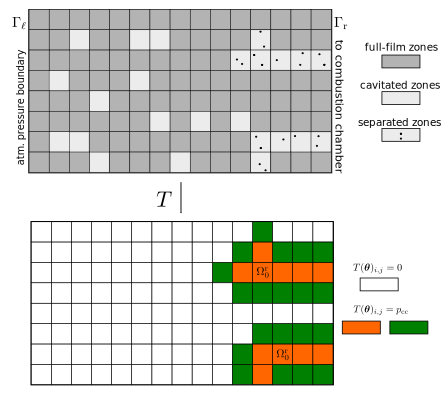
\includegraphics[scale=0.55]{operator_T_discrete}
		 \end{figure}
\end{minipage}
\end{frame}

\subsection{Numerical results}
\begin{frame}
\tableofcontents[
currentsection,
currentsubsection,
subsectionstyle=show/shaded/hide
]
\end{frame}
%=============================================================
\begin{frame}
\frametitle{Numerical results: A textured ring}\vspace*{0.5cm}
\begin{center}
\begin{minipage}{0.9\textwidth}
	\centering 
	\movie[autostart,loop]{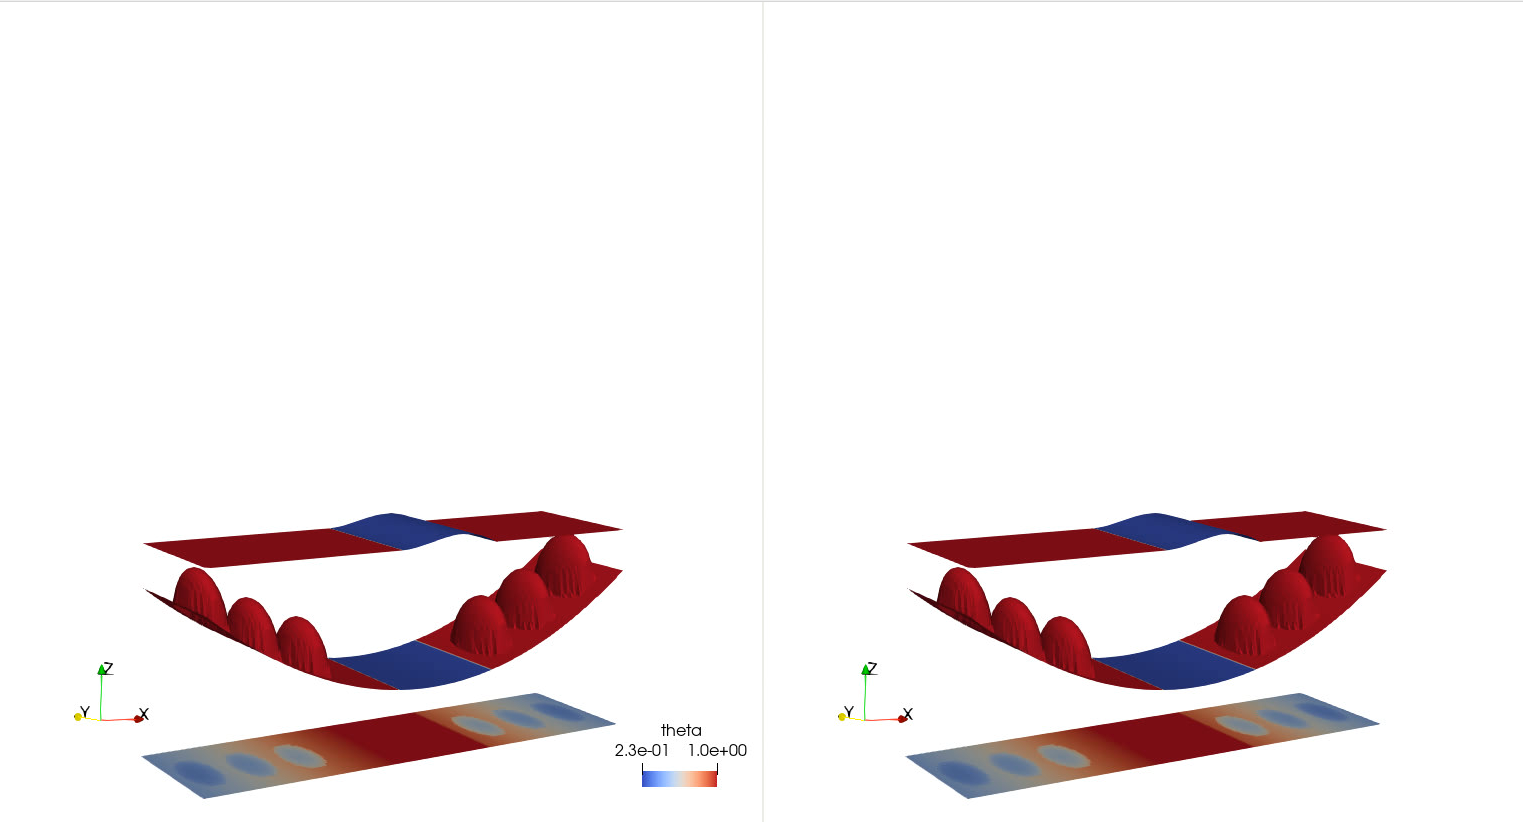
\includegraphics[width=\textwidth]{videos/0001.png}}{videos/videoa.ogv}
\end{minipage}
\end{center}

\end{frame}


%=============================================================
\begin{frame}
\frametitle{Numerical results: A textured ring}
\vspace*{1.0cm}
\begin{figure}
	\centering
	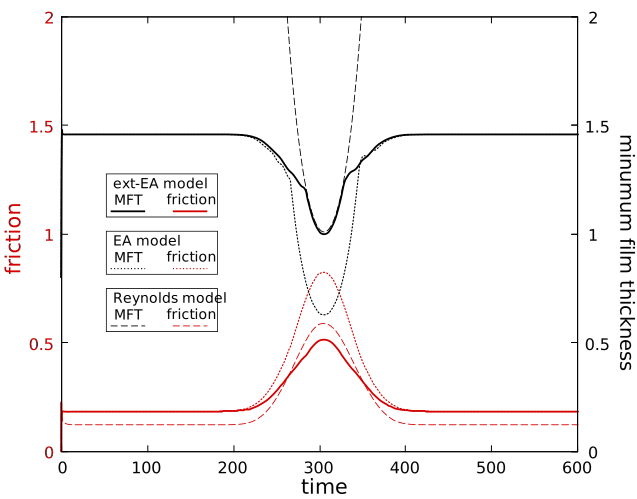
\includegraphics[scale=0.4]{friction_hmin_time}
\end{figure}
\end{frame}

%=============================================================
\begin{frame}
\frametitle{Numerical results: Blow-by}
\vspace*{1.0cm}
\begin{minipage}{0.5\textwidth}
	\begin{figure}
		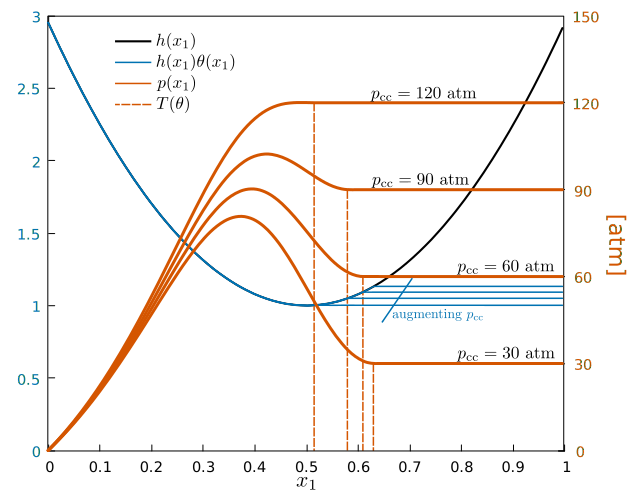
\includegraphics[scale=0.3]{stationary_cases}
	\end{figure}
\end{minipage}%
\begin{minipage}{0.5\textwidth}
	\begin{figure}
		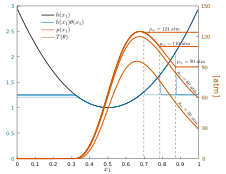
\includegraphics[scale=0.3]{stationary_cases2}
	\end{figure}
\end{minipage}

\end{frame}

%=============================================================
\begin{frame}
\frametitle{Numerical results: A ring with wear}
\vspace*{1.0cm}
\begin{figure}
	\centering
	\includegraphics[scale=0.65]{ring_wear}
\end{figure}
\end{frame}

%=============================================================
\begin{frame}
\frametitle{Numerical results: A ring with wear}

\begin{table}\centering {\small
		\begin{tabular}{cccccccccc}
			\toprule
			\multirow{2}{*}{} &
			
			\multicolumn{7}{c}{$\Delta h$} \\
			& 0.5 & 1.0& 1.5& 2.0 & 2.5& 3.0 & 3.5 &3.91& 4.0-8.0\\
			\midrule
			$\delta^\tm{max}$ & 0.025 &0.035 & 0.040 & 0.045 & 0.050 & 0.055 & 0.025& 0.005&0\\
			\bottomrule
	\end{tabular}}
	\caption{Minimum value of $\delta$ for which the simulations fail for every $\delta\geq \delta_\tm{max}$.}\label{tab:hmax}
\end{table}
\end{frame}

%=============================================================

\section{Well-posedness of the Reynolds-Rayleigh-Plesset coupling}

\begin{frame}
\tableofcontents[
currentsection,
currentsubsection,
subsectionstyle=show/shaded/hide
]
\end{frame}

%==============================================================
\begin{frame}
\frametitle{Motivation}
\begin{itemize}
	\item The Reynolds-Rayleigh-Plesset coupled system has been used in several numerical works to model cavitation along a flow equation (e.g., Navier-Stokes/Reynolds equations in the Software FLUENT).
	\item As far as we can tell, the well-posedness of this system has not been studied.
	\item There is a lack of robust numerical methods for solving it.
\end{itemize}
\end{frame}

\subsection{The Reynolds-Rayleigh-Plesset coupling}

%==============================================================
\begin{frame}
\frametitle{The Rayleigh-Plesset equation}
\vspace*{1.0cm}
\hspace*{-0.5cm}
\begin{minipage}{0.4\textwidth}
Knowing $p$ \emph{far away from} the bubble of radius $R$
\begin{equation*}
\overbrace{\rho_\ell\left(\frac{3}{2}\dot{R}^2+R\ddot{R}\right)}^{\text{inertial terms}}=\overbrace{p_b-p-\frac{2\sigma}{R}}^{\text{Young-Laplace eq.}}\overbrace{-\left(\mu_\ell+\frac{\kappa^s}{R}\right)\frac{4\dot{R}}{R}}^{\text{viscuous terms}}
\end{equation*}
\end{minipage}%
\hspace*{0.5cm}
\begin{minipage}{0.5\textwidth}
\begin{figure}[h]
	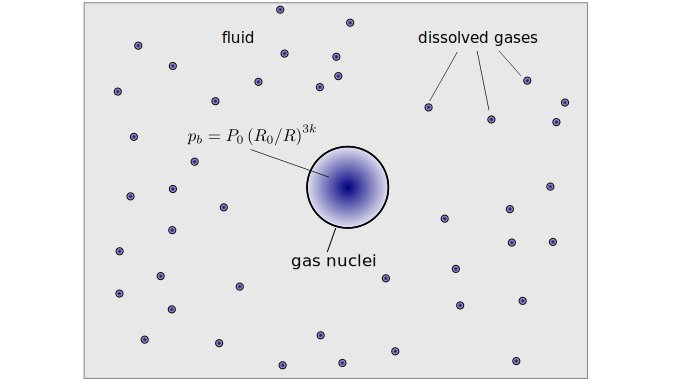
\includegraphics[scale=0.55]{gaseous_cavitation.pdf}
\end{figure}
\end{minipage}
\begin{center}
So we have the relation $p\longrightarrow R$
\end{center}

\end{frame}

%==============================================================
\begin{frame}
\frametitle{The Reynolds-Rayleigh-Plesset coupling}

To look for the fields $p(x,t)$ and $R(x,t)>0$ such that:
\begin{align*}
\nabla\cdot\left(\frac{\rho\left(\alpha\right) h^3}{12\mu\left(\alpha\right) }\nabla p \right)&=\frac{U}{2}\parder{\rho\left(\alpha\right) h}{x_1}+\parder{\rho\left(\alpha\right) h}{t},&&\alpha \longrightarrow p\\
\rho_\ell\left(\frac{3}{2}\dot{R}^2+R\ddot{R}\right)&=p_b-p-\frac{2\sigma}{R}-\left(\mu_\ell+\frac{\kappa^s}{R}\right)\frac{4\dot{R}}{R},&&p\longrightarrow R\\
\alpha&=\frac{\mbox{volume of gas}}{\mbox{volume of gas and liquid}}=\alpha\left(R\right),&&R\longrightarrow \alpha
\end{align*}
along suitable i.c. for $R$ and $\parder{R}{t}$.
\begin{center}
	Is this evolution the problem well-posed?\\
	Existence - uniqueness - stability
\end{center}
\end{frame} 

%==============================================================

\begin{frame}
\frametitle{The abstract problem: full RP equation}
To look for the fields $p(x,t)$ and $R(x,t)>0$ such that:
\begin{equation}
\underbrace{\frac{3}{2}\frac{1}{R}\left(\parder{R}{t}\right)^2+\frac{\partial^2 R}{\partial t^2}}_{\textnormal{inertial terms}}=\frac{f_1\left(R\right)-p}{R}-\parder{R}{t}f_2\left(R\right)\label{eq:abstract-rp1}
\end{equation}
and
\begin{align}
\begin{split}
\nabla_x\cdot \left(f_3\left(R\right) h^3\,\nabla p\right)&=\nabla_x\cdot \left(f_4\left(R\right)U\,h\,\right)+h\,f_5\left(R\right)\parder{R}{t},\\
p&=0 \qquad\mbox{on } \partial \Omega.
\end{split}
\label{eq:abstract-reynolds1}
\end{align}
Along suitable i.c. for $R$ and $\parder{R}{t}$.

\end{frame} 

%==============================================================

\begin{frame}
\frametitle{Well-posedness of the coupled system}
\begin{equation*}
	f_1\left(R\right)=p_b-p_\partial-\frac{2\sigma}{R},
\end{equation*}
\begin{align*}
f_2\left(R\right)&=4\left(\frac{\mu_\ell+\kappa^s/R}{R^2}\right),&f_3\left(R\right)&=\frac{1}{12}\frac{(1-\alpha\left(R\right))\rho_\ell+\alpha\left(R\right)\rho_g}{(1-\alpha\left(R\right))\mu_\ell+\alpha\left(R\right)\mu_g},\\ f_4\left(R\right)&=\frac{1}{2}\left[\rho_\ell+\alpha\left(R\right)\left(\rho_g-\rho_\ell\right)\right],&f_5\left(R\right)&=f_4'\left(\alpha\left(R\right)\right)\,\alpha'\left(R\right).
\end{align*}
\end{frame} 

%==============================================================

\begin{frame}
\frametitle{Well-posedness of the coupled system}
\begin{itemize}
	\item[H1:] $f_1\in C^2\left(\mathbb{R}^+_*;\mathbb{R}\right)$, ${\color{red}\exists \bar{R},\delta_1\in\mathbb{R}^+_*~\text{s.t.}~f_1\left(\bar{R}\right)=0~\text{and}~f'_1\left(R\right)<0\, \forall R \in [\bar{R}-\delta_1,\bar{R}+\delta_1];}$
	\item[H2:] $f_2\in C^2\left(\mathbb{R}_*^+;\mathbb{R}^+_*\right)$;
	\item[H3:] $f_3\in C^2\left(\mathbb{R}_*^+;\mathbb{R}\right)$ and $\exists m_3,M_3>0$ such that $m_3\leq f_3\left(r\right)\leq M_3$ $\forall r\in \mathbb{R}^+$;
	\item[H4:] $f_4\in C^2\left(\mathbb{R}_*^+;\mathbb{R}^+\right)$, $f_4'\left(r\right)<0$ $\forall r>0$;
	\item[H5:] $f_5\in C^2\left(\mathbb{R}_*^+;\mathbb{R}^-_*\right)$;
	\item[H6:] $h \in B_{m_0,M_0}$ for $0<m_0<M_0$ constants. Denoting $h_0=\underset{\Omega}{\essinf{\,h}}$.
\end{itemize}
With $B_{\alpha,\beta	}=\left\{w\in L^\infty\left(\Omega\right):\alpha \leq w \leq \beta\mbox{ a.e. on } \Omega \right\}.$
\end{frame} 

%==============================================================
\subsection{Local existence in time}
\begin{frame}
\tableofcontents[
currentsection,
currentsubsection,
subsectionstyle=show/shaded/hide
]
\end{frame}

%==============================================================

\begin{frame}
\frametitle{The abstract problem: full RP equation}
To look for the fields $p(x,t)$ and $R(x,t)>0$ such that:
\begin{equation*}
\frac{3}{2}\frac{1}{R}\left(\parder{R}{t}\right)^2+\frac{\partial^2 R}{\partial t^2}=\frac{f_1\left(R\right)-{\color{red}p}}{R}-\parder{R}{t}f_2\left(R\right)
\end{equation*}
and
\begin{align*}
\begin{split}
\nabla_x\cdot \left(f_3\left(R\right) h^3\,\nabla p\right)&=\nabla_x\cdot \left(f_4\left(R\right)U\,h\,\right)+h\,f_5\left(R\right)\parder{R}{t},\\
p&=0 \qquad\mbox{on } \partial \Omega.
\end{split}
\end{align*}

Along suitable i.c. for $R$ and $\parder{R}{t}$. Envisioning to use the Cauchy-Lipschitz Theorem, can we write
\begin{center}
 {\color{red}$p=A\left(R,\parder{R}{t}\right)$}?
\end{center}
\end{frame} 

%==============================================================

\begin{frame}
\frametitle{Well-posedness: local existence in time}
\vspace*{0.8cm}
Denoting $Q=\left\{R\in C\left(\bar{\Omega}\right):R>0\right\}$. We introduce the mapping
\begin{equation*}
\begin{array}{cccc}
A:&Q\times \cont&\longrightarrow& \cont\\
&(R_1,R_2)& \longrightarrow & A_1(R_1)+A_2\left(R_1,R_2\right),
\end{array}
\end{equation*}
where $A_1\left(R_1\right)$ is the unique solution of the elliptic problem
\begin{nalign}
\nabla\cdot \left(h^3f_3\left(R_1\right)\nabla A_1\left(R_1\right)\right)&=\nabla\cdot \left(U\,h\,f_4(R_1)\right)&&\textnormal{ in }\Omega,\\
A_1\left(R_1\right)&=0&&\textnormal{ on } \partial \Omega,
\label{eq:def-A1}
\end{nalign}
and $A_2\left(R_1,R_2\right)$ is the unique solution of the elliptic problem
\begin{equation}
\begin{aligned}
\nabla\cdot \left(h^3f_3\left(R_1\right)\nabla A_2\left(R_1,R_2\right)\right)&=h\,f_5\left(R_1\right)R_2
&&\textnormal{ in }\Omega,\\
A_2\left(R_1,R_2\right)&=0 &&\textnormal{ on } \partial \Omega.
\label{eq:def-A2}
\end{aligned}
\end{equation}
$A_1\left(R_1\right)$ and $A_2\left(R_1,R_2\right)$ are in $\cont$ due to a Sobolev compact embedding (Adams, 1975).
\end{frame} 

%==============================================================

\begin{frame}\frametitle{Well-posedness: local existence in time}
Then, the problem \eqref{eq:abstract-rp1}-\eqref{eq:abstract-reynolds1} can be rewritten as
\begin{equation}
\begin{split}
\frac{d\tilde{R}}{dt}&=F(\tilde{R}),\\
\tilde{R}(0)&=\tilde{R}_0,
\end{split}\label{eq:problem-rewritten}
\end{equation}
where $\tilde{R}=\left(R_1,R_2\right)=\left(R,\parder{R}{t}\right)$, $\tilde{R}_0=(r_1,r_2)\in Q\times \cont$ and $F:Q\times \cont\mapsto \left(\cont\right)^2$ with
\begin{equation}
F(R_1,R_2)=\left(
R_2,~-\frac{3}{2}\frac{R_2^2}{R_1}-R_2f_2\left(R_1\right)+\frac{f_1\left(R_1\right)-A\left(R_1,R_2\right)}{R_1}\right)
\end{equation}
Thus, the Cauchy-Lipschitz Theorem implies the local existence result:
\begin{theorem}There exists $T>0$ such that the  problem \eqref{eq:problem-rewritten} has a unique solution in $C^3\left([0,T];Q\times \cont\right)$.
\end{theorem}
\end{frame}

\begin{frame}
\frametitle{The simplified problem: disregarding inertial terms}
\vspace*{0.6cm}
\begin{equation}
\parder{R}{t}=\frac{f_1\left(R\right)-A\left(R,\parder{R}{t}\right)}{R\,f_2\left(R\right)}=\Pi\left(R,\parder{R}{t}\right)\label{eq:abstract-rp-inertialess},
\end{equation}
along the i.c. $R\left(\cdot,0\right)=r_1$ in $\Omega$.
Denoting $S=\parder{R}{t}$ we write
\begin{equation}
S=\frac{f_1\left(R\right)-A\left(R,S\right)}{R\,f_2\left(R\right)}=\Pi\left(R,S\right){\color{red}\overset{?}{=}G\left(R\right)}.
\end{equation}\vspace*{-0.5cm}
\begin{lemma}\label{lemma:fixed-point-Pi}
	Given $R\in Q$, there exists a unique $G\left(R\right)\in \cont$ such that
	$$G\left(R\right)=\Pi\left(R,G\left(R\right)\right),$$
	and the mapping $R\mapsto G\left(R\right)$ is of class $C^2$.
\end{lemma}
The proof is based in the Fredholm Alternative Theorem and the equivalence
$$S=\Pi\left(R,S\right)\Leftrightarrow S+\frac{A_2\left(R,S\right)}{Rf_2\left(R\right)}=\frac{f_1\left(R\right)-A_1\left(R\right)}{Rf_2\left(R\right)}.$$
\end{frame} 

%==============================================================

\begin{frame}\frametitle{Disregarding inertial terms}
\begin{theorem}There exists $T>0$ such that  problem \eqref{eq:abstract-reynolds1}-\eqref{eq:abstract-rp-inertialess} with i.c. $R\left(\cdot,0\right)=r_1$ in $\Omega$ has a unique solution in $C^3\left([0,T];Q\right)$.

\end{theorem}
The result follows directly from applying the Cauchy-Lipschitz Theorem to the equivalent evolution problem
\begin{equation}
\parder{R}{t}=G(R),\label{eq:ev-problem-G}
\end{equation}
along the initial condition written above.

\end{frame}

%==============================================================

\subsection{Stationary solutions: existence and stability}
\begin{frame}
\tableofcontents[
currentsection,
currentsubsection,
subsectionstyle=show/shaded/hide
]
\end{frame}

%==============================================================

\begin{frame}
\frametitle{The abstract problem: full RP equation}
To look for the fields $p(x,t)$ and $R(x,t)>0$ such that:
\begin{equation*}
\frac{3}{2}\frac{1}{R}\left(\parder{R}{t}\right)^2+\frac{\partial^2 R}{\partial t^2}=\frac{f_1\left(R\right)-p}{R}-\parder{R}{t}f_2\left(R\right)
\end{equation*}
and
\begin{align*}
\begin{split}
\nabla_x\cdot \left(f_3\left(R\right) h^3\,\nabla p\right)&=\nabla_x\cdot \left(f_4\left(R\right)U\,h\,\right)+h\,f_5\left(R\right)\parder{R}{t},\\
p&=0 \qquad\mbox{on } \partial \Omega.
\end{split}
\end{align*}

Along suitable i.c. for $R$ and $\parder{R}{t}$.


\end{frame} 

%==============================================================

\begin{frame}
\frametitle{The stationary problem}

Observe that a stationary solution $(R_s,p_s)$ of problem \eqref{eq:abstract-rp1}-\eqref{eq:abstract-reynolds1} satisfies
\begin{equation}
p_s=f_1\left(R_s\right).\label{eq:p_s}
\end{equation}
Writing $h=h_0+h^+$ with $h_0=\underset{\Omega}{\essinf{\,h}}$, $(R_s,p_s)$ is solution of the system
\begin{nalign}
	\nabla\cdot \left(\left(h_0+h^+\right)^3f_3\left(R_s\right)\nabla p_s\right)&=\nabla\cdot\left(U\left(h_0+h^+\right)f_4\left(R_s\right)\right)&&\textnormal{ in } \Omega,\\
	p_s&=f_1\left(R_s\right)&&\textnormal{ in } \Omega,\\
	R_s&>0&&\textnormal{ in } \Omega,\\
	p_s&=0&&\textnormal{ on }\partial \Omega.
	\label{eq:problem-stationary}
\end{nalign}
Observe that if $U=0$ or $h^+=0$ then $\left(R_s,p_s\right)=\left(\bar{R},0\right)$ is solution of \eqref{eq:problem-stationary}.


\end{frame} 

\begin{frame}
\frametitle{The stationary problem}

\begin{figure}[h]
	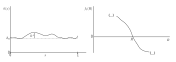
\includegraphics[scale=0.85]{drawing_h_f1.pdf}
\end{figure}

\end{frame} 

%==============================================================

\begin{frame}
\frametitle{Stationary solutions: existence}
\begin{theorem}\label{theo:existence_U_fix}
	Fix $U\in\mathbb{R}^2$ and $h_0>0$. Then there exists $\epsilon\left(U\right)>0$ such that the problem \eqref{eq:problem-stationary} has a unique solution $\left(R_s,p_s\right)$ with $R_s>0$ whenever $\norm{h^+}{\infty}<\epsilon(U)$.\\ {\color{red}Moreover, the solution $\left(R_s,p_s\right)$ depends continuously on $h^+$}.
\end{theorem}
\begin{theorem}\label{theo:existence_h_fix}
	Fix $h\in B_{m_0,M_0}$, $0<m_0<M_0$. Then there exists $\epsilon\left(h\right)>0$ such that the problem \eqref{eq:problem-stationary} has a unique solution $\left(R_s,p_s\right)$ with $R_s>0$ whenever $\norm{U}{}<\epsilon\left(h\right)$.\\  {\color{red}Moreover, the solution $\left(R_s,p_s\right)$ depends continuously on $U$}.
\end{theorem}
\bigskip

We will show a scheme of the proof for Theorem 2, Theorem 3 follows analogously.
\end{frame} 

%==============================================================
\begin{frame}
\frametitle{Proof of Theorem \ref{theo:existence_U_fix}, $U$ fixed}
\vspace*{0.6cm}
Since $\nabla p_s=f_1'\left(R_s\right)\nabla R_s$ the problem \eqref{eq:problem-stationary} can be written in function of $\xi$ as
\begin{nalign}
	-\nabla\cdot \left(\left(h^++h_0\right)^3a_0\left(\xi\right)\nabla\,\xi\right)&=\nabla\cdot \left(U h^+\,b_0(\xi)\right)+\nabla\cdot \left(Uh_0\,b_0(\xi)\right)&&\textnormal{ in }\Omega,\\
	\xi&>-\bar{R}&&\textnormal{ in }\Omega,\\
	\xi&=0&&\textnormal{ on } \partial \Omega,
	\label{eq:problem-stationary-change}
\end{nalign}
where $a_0\left(\xi\right)=-f_3\left(\bar{R}+\xi\right)f_1'\left(\bar{R}+\xi\right)$, and $b_0(\xi)=f_4\left(\bar{R}+\xi\right)$. We introduce the open set
$$W=\left\{\xi\in W_0^{1,q}\left(\Omega\right):\xi >-\bar{R}\textnormal{ a.e. on } \Omega\right\},$$
and the application $\phi:W\times L^\infty\left(\Omega\right)\longmapsto W^{-1,q}$:
\begin{equation}
\phi(\xi,\delta) =  \nabla\cdot \left(\left(\delta+h_0\right)^3a_0\left(\xi\right)\nabla\,\xi\right)+\nabla\cdot \left(U\delta\,b_0(\xi)\right)+\nabla\cdot \left(Uh_0\,b_0(\xi)\right),
\end{equation}
since $\phi(0,0)=0$ and $\partial_\xi\phi(0,0)$ is invertible, the Implicit Function Theorem implies that there exists $\xi=\xi\left(\delta\right)\Leftrightarrow R_s=R_s\left(h^+\right)$ {\color{red}smooth}.
\end{frame}

%==============================================================

\begin{frame}
\frametitle{Stability with inertial terms}
\vspace*{0.5cm}
\begin{equation}
\begin{split}
\frac{d\tilde{R}}{dt}&=F(\tilde{R}),\\
\tilde{R}(0)&=\tilde{R}_0,
\end{split}
\end{equation}
where $\tilde{R}_0=\begin{pmatrix}
{r}_1\\ {r}_2
\end{pmatrix}\in Q$ and $F:Q\times \cont\mapsto \left(\cont\right)^2$ with
\begin{equation}
F(R_1,R_2)=\left(
R_2,~-\frac{3}{2}\frac{R_2^2}{R_1}-R_2f_2\left(R_1\right)+\frac{f_1\left(R_1\right)-A\left(R_1,R_2\right)}{R_1}\right)
\end{equation}
We denote by $\mathcal{L}_F$ the Fréchet derivative of $F$ at $\left(R_1,R_2\right)=\left(R_s,0\right)$, i.e.,
\begin{equation}
\begin{array}{cccl}
\mathcal{L}_F:&\left(\cont\right)^2&\longmapsto& \left(\cont\right)^2\\
&(S_1,S_2)& \longmapsto & D\,F\left(R_s,0\right)\left(S_1,S_2\right).\label{eq:jacobian_inertia}
\end{array}
\end{equation} 
It is shown that, for some particular cases, the spectrum of $\mathcal{L}_F$ is such that $$\mbox{Re}\left(\lambda\right)<0\qquad \forall \lambda\in \Sp{\mathcal{L}_F}.$$
\end{frame}

%==============================================================

\begin{frame}
\frametitle{Stability with inertial terms}\vspace*{0.5cm}
We compute $\mathcal{L}_F$ for the cases $h^+=0$ or $U=0$, obtaining
\begin{equation}\label{eq:L_F}
\mathcal{L}_F\left(S_1,S_2\right)=B\begin{pmatrix}
S_1\\S_2
\end{pmatrix}-b_r\begin{pmatrix}
0\\\pi_1\left(S_1\right)+\pi_2\left(S_2\right)
\end{pmatrix},
\end{equation}
where $B=\begin{pmatrix}0&1\\-b_1&-b_2
\end{pmatrix}$, $\pi_1(S_1)$ is the solution of:
\begin{nalign}
	-b_3\nabla\cdot \left(h^3 \,\nabla \pi_1\left(S_1\right)\right)&=b_4\nabla\cdot \left(UhS_1\right)&&\textnormal{ in }  \Omega,\\
	\pi_1\left(S_1\right)&=0 &&\textnormal{ on } \partial \Omega,
	\label{eq:pi1-triv-case}
\end{nalign}
and $\pi_2(S_1)$ is the solution of:
\begin{nalign}
	-\nabla\cdot \left(h^3f_3\left(R_s\right) \,\nabla \pi_2\left(S_2\right)\right)&=-hf_5\left(R_s\right)S_2&&\textnormal{ in }  \Omega,\\
	\pi_2\left(S_2\right)&=0 &&\textnormal{ on } \partial \Omega.
	\label{eq:def:pi2}
\end{nalign}
We denote by $\{\lambda_1^B,\lambda_2^B\}$ the set of eigenvalues of $B$ and notice that $\mbox{Re}\left(\lambda_1^B\right)<0$ and $\mbox{Re}\left(\lambda_2^B\right)<0$.
\end{frame}

%==============================================================

\begin{frame}
\frametitle{Stability with inertial terms}
\begin{lemma}\label{lemma:spec-L_F}
	Let $h^+=0$ or $U=0$. Then
	\begin{equation}
	\Sp{\mathcal{L}_F}\subset \Vp{\mathcal{L}_F}\cup \{\lambda_1^B,\lambda_2^B\}.
	\end{equation}
	Moreover if $\lambda\in \Vp{\mathcal{L}_F}\setminus\{\lambda_1^B,\lambda_2^B\}$ with associated eigenfunction $\left(S_1,S_2\right)\in\cont^2$ then $\left(S_1,S_2\right)\in\hzero^2$, $S_2=\lambda S_1$ and $S_1$ is solution of the problem
	\begin{align*}
	\frac{b_3}{b_r}\xi\left(\lambda\right)\nabla\cdot\left(h^3\nabla S_1\right)&=b_4 U\cdot\nabla\left(hS_1\right)+\lambda\, b_5 h\, S_1 && \textnormal{in }\Omega,\\
	S_1&=0&&\textnormal{on }\partial\Omega,
	\end{align*}
	where $\xi\left(\lambda\right)=\lambda^2+b_2\lambda+b_1$ with roots $\{\lambda_1^B,\lambda_2^B\}$.
\end{lemma}
The first part of the proof is based in the fact that from Eq. \eqref{eq:L_F} we have (for any $\lambda\in \mathbb{C}\setminus \{\lambda_1^B,\lambda_2^B\}$)
\begin{equation*}
\left(\mathcal{L}_F-\lambda I\right)\begin{pmatrix}
S_1\\S_2
\end{pmatrix}=\left(B-\lambda I\right)\left[\begin{pmatrix}
S_1\\S_2
\end{pmatrix}-b_r\left(B-\lambda I\right)^{-1}
\begin{pmatrix}
0\\ \pi_1\left(S_1\right)+\pi_2\left(S_2\right)
\end{pmatrix}	
\right].\label{eq:vp-L}
\end{equation*}	
\end{frame}

%==============================================================

\begin{frame}
\frametitle{Stability with inertial terms}
\begin{theorem}\label{theo:stabilite-avec-inertie-h-fixe} Let $h\in B_{m_0,M_0}$, $0<m_0<M_0$ (as in Theorem \ref{theo:existence_h_fix}). Then there exists $\epsilon\left(h\right)>0$ s.t. if $\norm{U}{\infty}<\epsilon$ the solution $\left(R_s,p_s\right)$ of problem \eqref{eq:problem-stationary} is asymptotically stable for the evolution problem \eqref{eq:problem-rewritten}.
\end{theorem}
Take first $U=0$. From Lemma \ref{lemma:spec-L_F} it is enough to study $\Vp{\mathcal{L}_F}$. Thus, take $\lambda\in \Vp{\mathcal{L}_F}\setminus\{\lambda_1^B,\lambda_2^B\}$ with associated eigenfunction $\left(S_1,S_2\right)$. From the same lemma, $S_1\in \hzero$ accomplishes the next variational formulation\footnote{it can be shown that $\lambda\neq 0$}
\begin{equation}\small
-\frac{b_3}{b_r}\frac{\xi\left(\lambda\right)}{\lambda}\int_\Omega h^3 \nabla S_1\nabla \phi\,d\Omega=b_5\int_\Omega h S_1\,\phi\,d\Omega\qquad \forall \phi \in \hzero.
\end{equation}
Taking $\phi=S_1$ we obtain that $\gamma=-\xi\left(\lambda\right)/\lambda\in \mathbb{R}^+$ , from where we conclude that $\mbox{Re}\left(\lambda\right)<0$. 

{\color{red}From Theorem \ref{theo:existence_h_fix}}, the mapping $U\mapsto R_s\left(U\right)$ is continuous in a neighborhood $V_1\ni 0$ in $\mathbb{R}^2$, thus if $U\rightarrow 0$ in $\mathbb{R}^2$ then $\norm{DF\left(R_s\left(U\right),0\right)-DF\left(\bar{R},0\right)}{}\rightarrow 0$ in the space of linear continuous operators from $\cont^2$ into itself. This, plus the continuity of the spectrum give us the result.
\end{frame}

%==============================================================

\begin{frame}
\frametitle{Stability with inertial terms}
\begin{theorem}\label{theo:instabilite-avec-inertie-U-fixe} Set $h^+=0$ and consider the one-dimensional case ($N=1$). Then there exists $M>0$ such that if $\norm{U}{\infty}>M$ the solution $\left(R_s,p_s\right)$ of problem \eqref{eq:problem-stationary} is asymptotically unstable for the evolution problem \eqref{eq:problem-rewritten}.
\end{theorem}
The proof is based in showing that there exists $\lambda\in \Vp{\mathcal{L}_F}$ such that $\mbox{Re}(\lambda)>0$ for $U$ big enough.
\end{frame}

%==============================================================

\begin{frame}\frametitle{Stability without inertial terms}
Recalling the evolution problem
\begin{equation}
\parder{R}{t}=G(R)=\Pi\left(R,G\left(R\right)\right),
\end{equation}
with i.c. $R\left(\cdot,0\right)=r_1$ in $\Omega$. We denote the derivative
\begin{equation}
\begin{array}{cccl}
\mathcal{L}_G:&\cont&\longmapsto& \cont\\
&w& \longmapsto & D\,G\left(R_s\right)\left(w\right).\label{eq:def-L_G}
\end{array}
\end{equation} 
\bigskip

Notice that the existence theorems (\ref{theo:existence_U_fix}) and (\ref{theo:existence_h_fix}) for solutions of the stationary problem are still valid when disregarding the inertial terms.
\end{frame}

%==============================================================

\begin{frame}\frametitle{Stability without inertial terms}
\begin{lemma}\label{lemma:spec-L_G}
Asumme $h^+=0$ or $U=0$. Then 
$$\Sp{\mathcal{L}_G}\subset\Vp{\mathcal{L}_G}\cup\{-d_1\}.$$
Moreover, if $w\in\cont$ is an eigenvector of $\mathcal{L}_G$ with associated eigenvalue $\lambda$, then $w\in\hzero$ and it satisfies 
\begin{nalign}
	\begin{split}
		d_3\left(d_1+\lambda\right)\nabla\cdot \left(h^3\nabla w\right)&=d_4\,U\cdot \nabla \left(hw\right)+\lambda \,d_5\,hw&&\textnormal{ in } \partial \Omega,\\
		w&=0 &&\textnormal{ on } \partial \Omega.
	\end{split}
	\label{eq:eigenvectors-L_G}
\end{nalign}
\end{lemma}
In this case we have $\left(R_s,p_s\right)=\left(\bar{R},0\right)$, so we can show that
we obtain that for any $\lambda\in\mathbb{C}$:
\begin{equation}
\mathcal{L}_G\left(w\right)-\lambda\, w=\left(\lambda+d_1\right)\left[-w-\frac{d_2}{\lambda+d_1}\left[\pi_1\left(w\right)+\pi_2\left(\mathcal{L}_G\left(w\right)\right)\right]\right],\label{eq:L_G2}
\end{equation}
with $\pi_1\left(w\right)$ given by \eqref{eq:pi1-triv-case}.
\end{frame}

%==============================================================

\begin{frame}\frametitle{Stability without inertial terms}
\begin{theorem} \label{theo:stability-sans-inertie-h-fix}
	Fix $h\in B_{m_0,M_0}$, $0<m_0<M_0$. Then there exists $\epsilon>0$ s.t. if $\norm{U}{}<\epsilon$ then the solution $\left(R_s,p_s\right)$ of problem \eqref{eq:problem-stationary} is asymptotically stable for the evolution problem \eqref{eq:abstract-reynolds1}-\eqref{eq:abstract-rp-inertialess} along the i.c. $R\left(\cdot,0\right)=r_1$ in $\Omega$
\end{theorem}
\begin{theorem}\label{theo:stability-sans-inertie-U-fixe} For every $U\in \mathbb{R}^2$ there exists $\epsilon=\epsilon\left(U\right)>0$ s.t. if $\norm{h^+}{\infty}<\epsilon$, then the solution $\left(R_s,p_s\right)$ of problem \eqref{eq:problem-stationary} is asymptotically stable for the evolution problem \eqref{eq:abstract-reynolds1}-\eqref{eq:abstract-rp-inertialess} along the i.c. $R\left(\cdot,0\right)=r_1$ in $\Omega$
\end{theorem}

The proofs of these theorems are analogous to the one of theorem \ref{theo:stabilite-avec-inertie-h-fixe}, i.e., we show that $\mbox{Re}\left(\lambda\right)<0~\forall \lambda\in \Vp{\mathcal{L}_F}.$\\
\bigskip
Recall that there is no an analogous result of Theorem \ref{theo:stability-sans-inertie-U-fixe} for the case including the inertial terms!
\end{frame}

%==============================================================

\section{Numerical methods for the Reynolds-Rayleigh-Plesset coupling}
\subsection{Analysis without inertial terms}
\begin{frame}
\tableofcontents[
currentsection,
currentsubsection,
subsectionstyle=show/shaded/hide
]
\end{frame}
%==============================================================
\subsection{Analysis with inertial terms}
\begin{frame}
\tableofcontents[
currentsection,
currentsubsection,
subsectionstyle=show/shaded/hide
]
\end{frame}

%==============================================================
\begin{frame}\frametitle{Thank you for your attention!}\centering
\begin{center}
e-mail: ajaramil at icmc.usp.br
\end{center}

\end{frame}
%==============================================================



\end{document} 